\documentclass{../../slides-style}

\slidetitle{Паттерны и архитектурные стили}{12.07.2023}

\begin{document}

    \begin{frame}[plain]
        \titlepage
    \end{frame}

    \section{Введение}

    \begin{frame}
        \frametitle{Паттерны проектирования}
        \textbf{Шаблон проектирования} --- это повторимая архитектурная конструкция, являющаяся решением некоторой типичной технической проблемы
        \begin{itemize}
            \item Подходит для класса проблем
            \item Обеспечивает переиспользуемость знаний
            \item Позволяет унифицировать терминологию
            \item В удобной для изучения форме
            \item НЕ конкретный рецепт или указания к действию
        \end{itemize}
    \end{frame}
 
    \begin{frame}
        \frametitle{Архитектурные стили}
        Архитектурный стиль --- набор решений, которые
        \begin{enumerate}
            \item применимы в выбранном контексте разработки,
            \item задают ограничения на принимаемые архитектурные решения, специфичные для определённых систем в этом контексте,
            \item приводят к желаемым положительным качествам получаемой системы.
        \end{enumerate}
        Архитектурные шаблоны более <<стратегичны>> и более размыты, чем паттерны
    \end{frame}

    \begin{frame}
        \frametitle{Паттерны и архитектурные стили}
        \begin{center}
            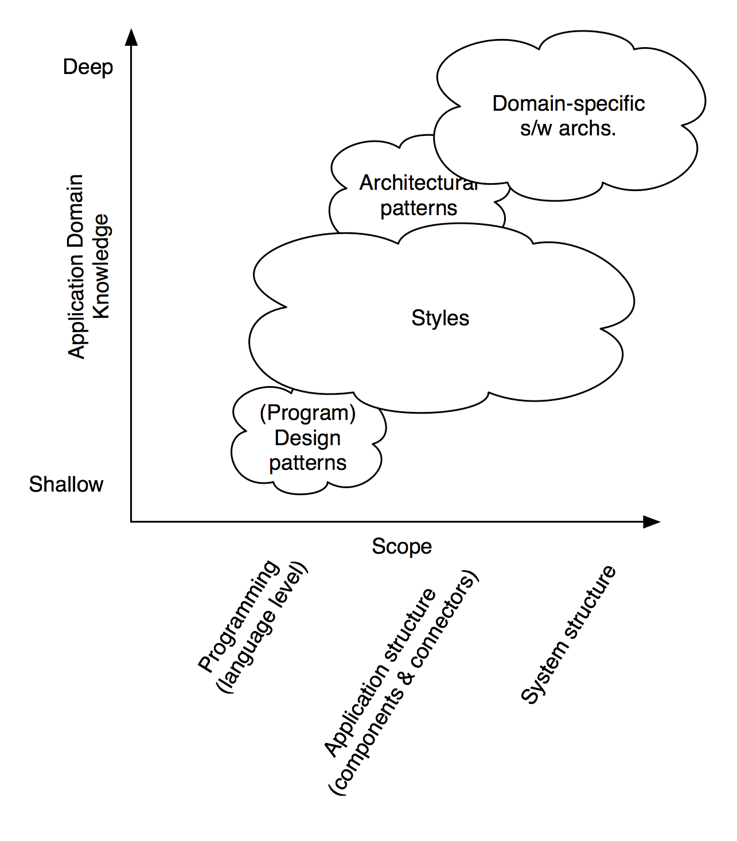
\includegraphics[width=0.5\textwidth]{architecturalStyles.png}
            \attribution{N. Medvidovic}
        \end{center}
    \end{frame}

    \begin{frame}
        \frametitle{Книжка про паттерны}
        \begin{columns}
            \begin{column}{0.6\textwidth}
                Приемы объектно-ориентированного проектирования. Паттерны проектирования

                Э. Гамма, Р. Хелм, Р. Джонсон, Дж. Влиссидес

                Design Patterns: Elements of Reusable Object-Oriented Software
            \end{column}
            \begin{column}{0.4\textwidth}
                \begin{center}
                    
\includegraphics[width=0.8\textwidth]{patternBookCover.png}
                \end{center}
            \end{column}
        \end{columns}
    \end{frame}

    \begin{frame}
        \frametitle{Пример: Model-View-Controller}
        \begin{center}
            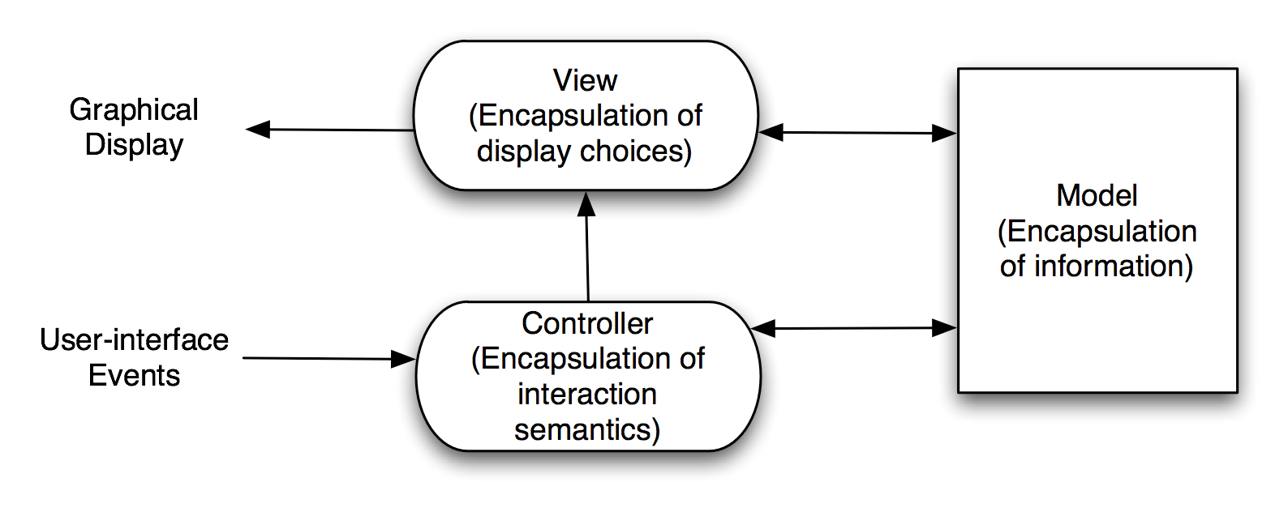
\includegraphics[width=0.65\textwidth]{mvc.png}
            \attribution{N. Medvidovic}
        \end{center}
        \begin{itemize}
            \item Разделяет данные, представление и взаимодействие с пользователем
            \item Если в модели что-то меняется, она оповещает представление (представления)
            \item Через контроллер проходит всё взаимодействие с пользователем
            \begin{itemize}
                \item Естественное место для паттерна <<Команда>> и Undo/Redo
            \end{itemize}
        \end{itemize}
    \end{frame}

    \section{Паттерны проектирования}

    \subsection{Паттерн <<Команда>>}

    \begin{frame}
        \frametitle{Паттерн <<Команда>>, мотивация}
        \begin{itemize}
            \item Хотим отделить инициацию запроса от его исполнения
            \item Хотим, чтобы тот, кто <<активирует>> запрос, не знал, как он исполняется
            \item При этом хотим, чтобы тот, кто знает, когда исполнится запрос, не знал, когда он будет активирован
            \item Но зачем?
            \begin{itemize}
                \item Команды меню приложения
                \item Палитры инструментов
                \item ...
            \end{itemize}
            \item Просто вызвать действие не получится, вызов функции жёстко свяжет инициатора и исполнителя
        \end{itemize}
    \end{frame}

    \begin{frame}
        \frametitle{Решение: обернём действие в объект}
        \begin{center}
            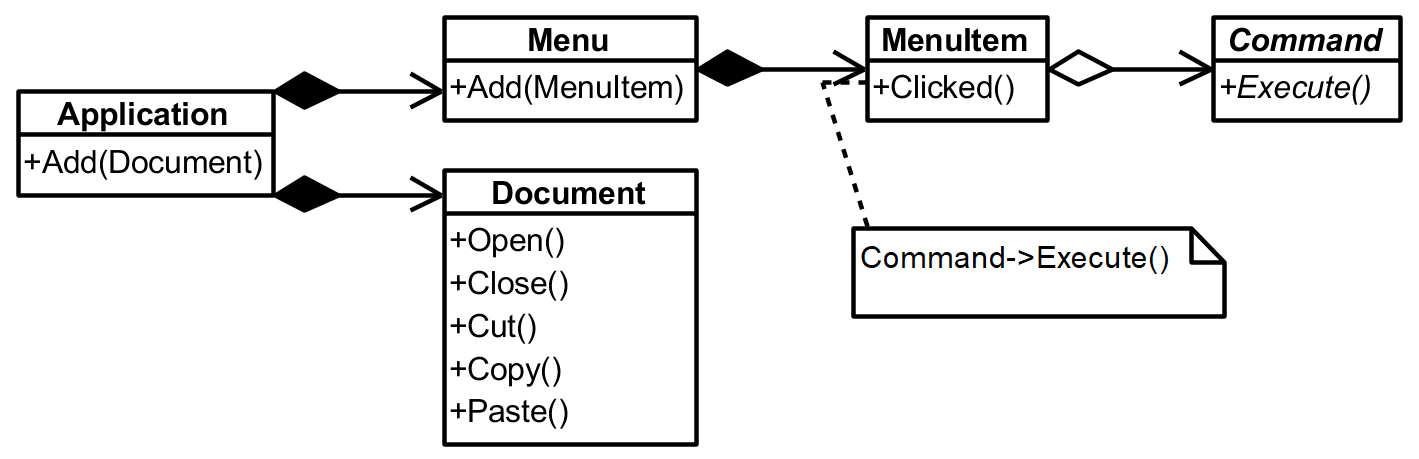
\includegraphics[width=0.9\textwidth]{commandExample.png}
        \end{center}
    \end{frame}

    \begin{frame}
        \frametitle{Команда вставки}
        \begin{center}
            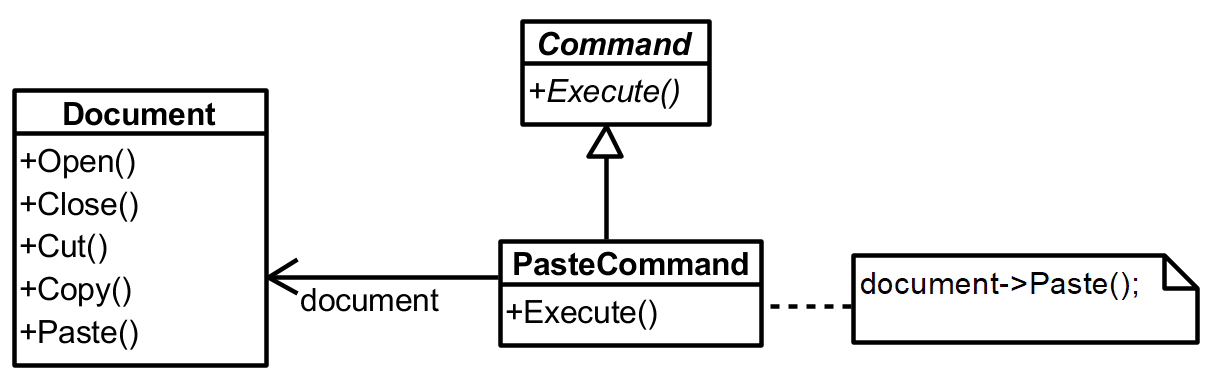
\includegraphics[width=0.75\textwidth]{pasteCommand.png}
        \end{center}
    \end{frame}

    \begin{frame}
        \frametitle{Команда открытия документа}
        \begin{center}
            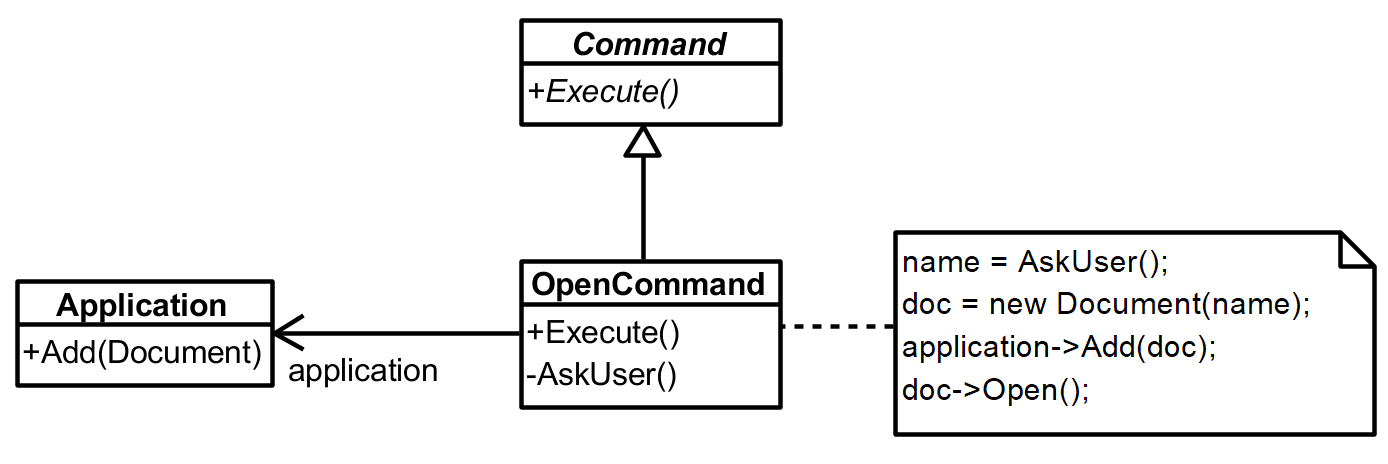
\includegraphics[width=0.75\textwidth]{openDocumentCommand.png}
        \end{center}
    \end{frame}

    \begin{frame}
        \frametitle{Составная команда}
        \begin{center}
            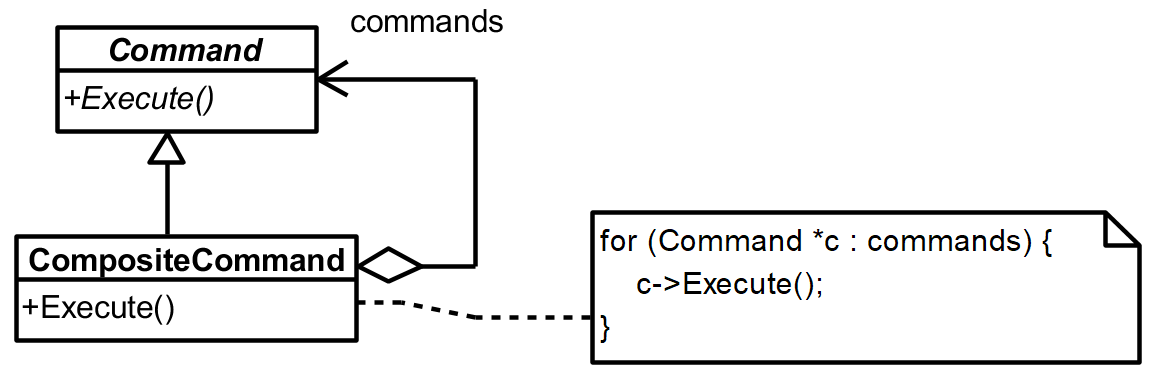
\includegraphics[width=0.75\textwidth]{compositeCommand.png}
        \end{center}
    \end{frame}

    \begin{frame}
        \frametitle{Паттерн <<Команда>>}
        \begin{center}
            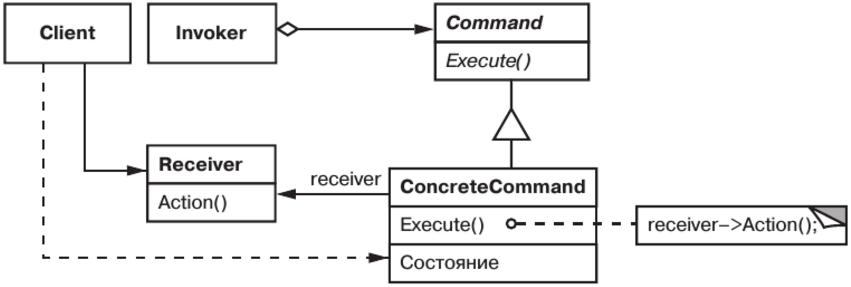
\includegraphics[width=0.9\textwidth]{command.png}
        \end{center}
    \end{frame}

    \begin{frame}
        \frametitle{Взаимодействие объектов}
        \begin{center}
            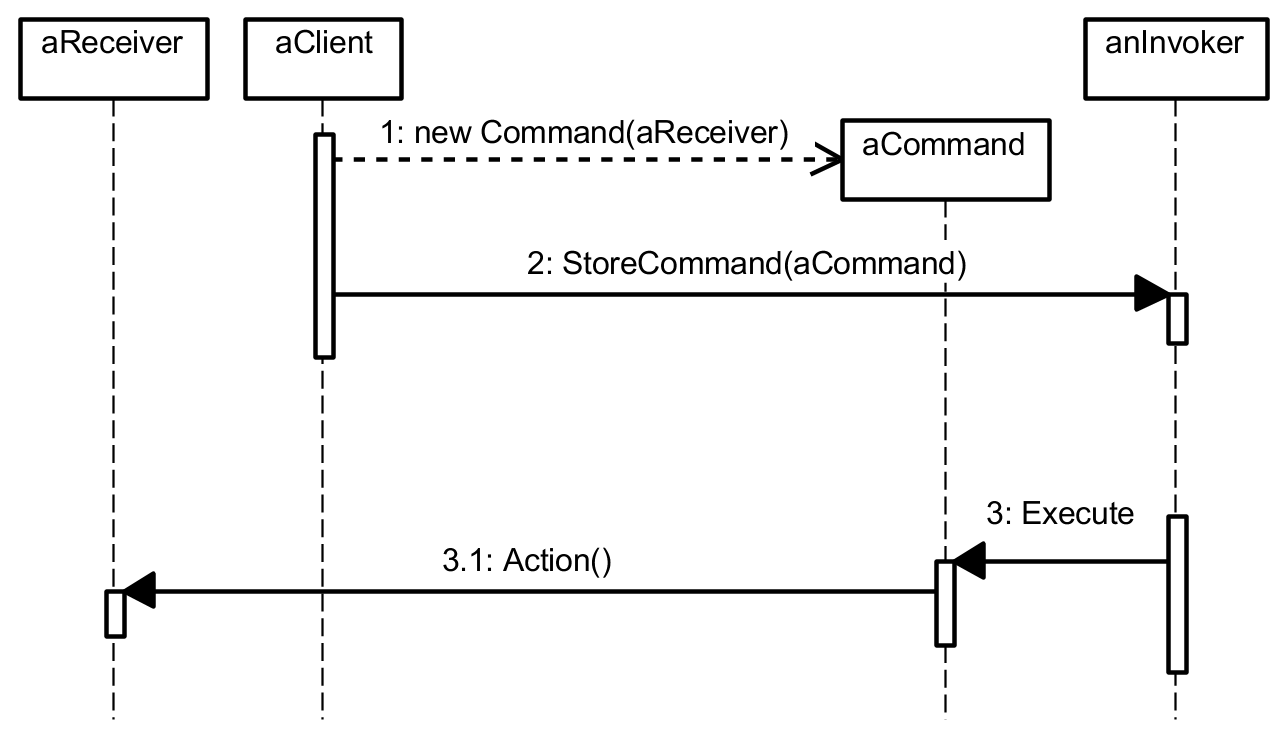
\includegraphics[width=0.9\textwidth]{commandSequence.png}
        \end{center}
    \end{frame}

    \begin{frame}
        \frametitle{Команда, применимость}
        \begin{itemize}
            \item Параметризовать объекты выполняемым действием
            \item Определять, ставить в очередь и выполнять запросы в разное время
            \item Поддержать отмену операций
            \item Структурировать систему на основе высокоуровневых операций, построенных из примитивных
            \item Поддержать протоколирование изменений
        \end{itemize}
    \end{frame}

    \begin{frame}
        \frametitle{<<Команда>> (Command), детали реализации}
        \begin{itemize}
            \item Насколько <<умной>> должна быть команда
            \item Отмена и повторение операций --- тоже от хранения всего состояния в команде до <<вычислимого>> отката
            \begin{itemize}
                \item Undo-стек и Redo-стек
                \item Может потребоваться копировать команды
                \item Искусственные команды
                \item Композитные команды
            \end{itemize}
        \end{itemize}
    \end{frame}

    \begin{frame}[fragile]
        \frametitle{<<Команда>>, пример}
        \begin{itemize}
            \item Qt, класс QAction:
            \begin{minted}{c++}
const QIcon openIcon = QIcon(":/images/open.png");
QAction *openAct = new QAction(openIcon, tr("&Open..."), this);

openAct->setShortcuts(QKeySequence::Open);
openAct->setStatusTip(tr("Open an existing file"));

connect(openAct, &QAction::triggered, this, &MainWindow::open);

fileMenu->addAction(openAct);
fileToolBar->addAction(openAct);
            \end{minted}
            \item ICommand в .NET
        \end{itemize}
    \end{frame}

    \subsection{Паттерн <<Абстрактная фабрика>>}

    \begin{frame}
        \frametitle{<<Абстрактная фабрика>>, мотивация}
        \begin{itemize}
            \item Хотим поддержать разные стили UI
            \begin{itemize}
                \item Гибкая поддержка в архитектуре
                \item Удобное добавление новых стилей
            \end{itemize}
        \end{itemize}
        \begin{center}
            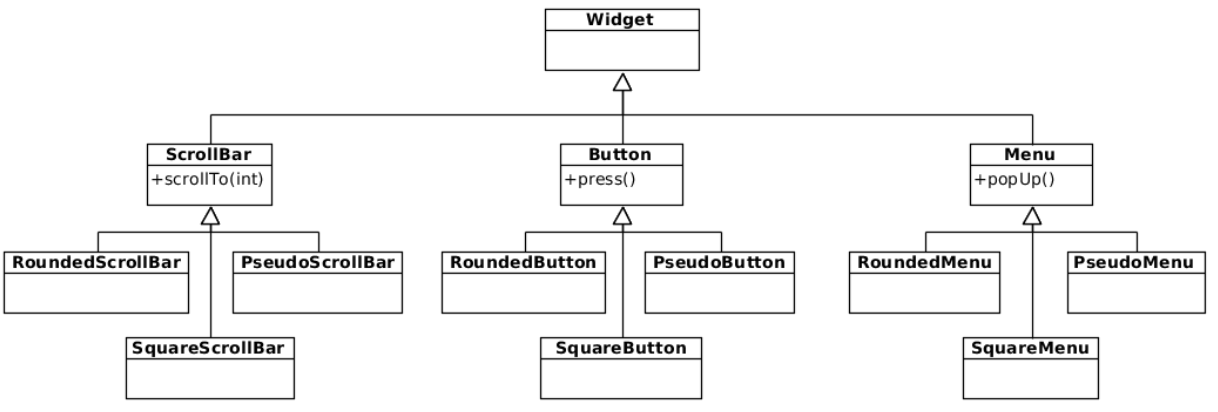
\includegraphics[width=0.95\textwidth]{widgets.png}
        \end{center}
    \end{frame}

    \begin{frame}
        \frametitle{Создание виджетов}
        \mintinline{c++}|ScrollBar* bar = new RoundedScrollBar;|
        
        \vspace{2mm}
        
        vs
        
        \vspace{2mm}
        
        \mintinline{c++}|ScrollBar* bar = guiFactory->createScrollBar();|
    \end{frame}

    \begin{frame}
        \frametitle{Фабрика виджетов}
        \begin{center}
            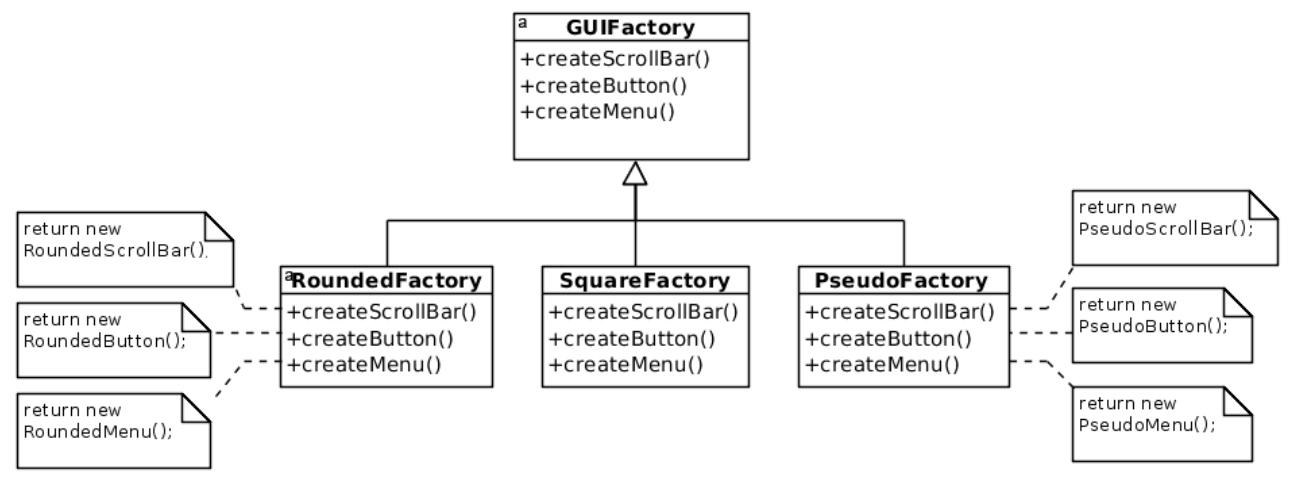
\includegraphics[width=0.95\textwidth]{widgetFactory.png}
        \end{center}
    \end{frame}

    \begin{frame}
        \frametitle{Паттерн <<Абстрактная фабрика>>}
        \framesubtitle{Abstract Factory}
        \begin{columns}
            \begin{column}{0.4\textwidth}
                \begin{itemize}
                    \item Изолирует конкретные классы
                    \item Упрощает замену семейств продуктов
                    \item Гарантирует сочетаемость продуктов
                    \item Поддержать новый вид продуктов непросто
                \end{itemize}
            \end{column}
            \begin{column}{0.6\textwidth}
                \begin{center}
                    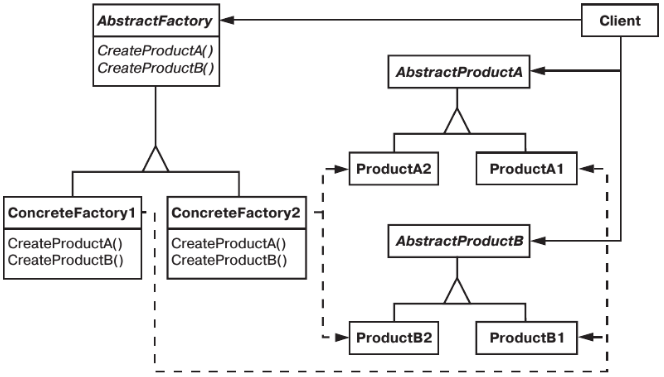
\includegraphics[width=0.95\textwidth]{abstractFactory.png}
                \end{center}
            \end{column}
        \end{columns}
    \end{frame}

    \begin{frame}
        \frametitle{<<Абстрактная фабрика>>, детали реализации}
        \begin{columns}
            \begin{column}{0.5\textwidth}
                \begin{itemize}
                    \item Хорошо комбинируются с паттерном <<Одиночка>>
                    \item Если семейств продуктов много, то фабрика может инициализироваться \textit{прототипами}, тогда не надо создавать сотню подклассов
                \end{itemize}
            \end{column}
            \begin{column}{0.5\textwidth}
                \begin{center}
                    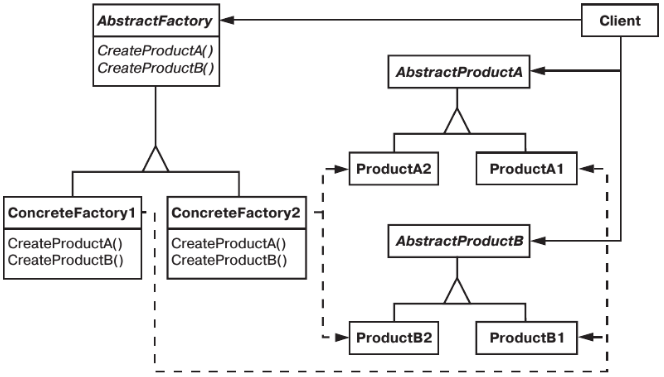
\includegraphics[width=\textwidth]{abstractFactory.png}
                \end{center}
            \end{column}
        \end{columns}
        \begin{itemize}
            \item Прототип на самом деле может быть классом (например, Class в Java)
            \item Часто это просто лямбда, создающая объект
            \item Если виды объектов часто меняются, может помочь параметризация метода создания
        \end{itemize}
    \end{frame}

    \subsection{Паттерн <<Заместитель>>}

    \begin{frame}
        \frametitle{Управление доступом к объектам}
        \begin{itemize}
            \item Встраивание в документ графических объектов
            \begin{itemize}
                \item Затраты на создание могут быть значительными
                \item Хотим отложить их на момент использования
            \end{itemize}
            \item Использование заместителей объектов
        \end{itemize}
        \vspace{3mm}
        \begin{center}
            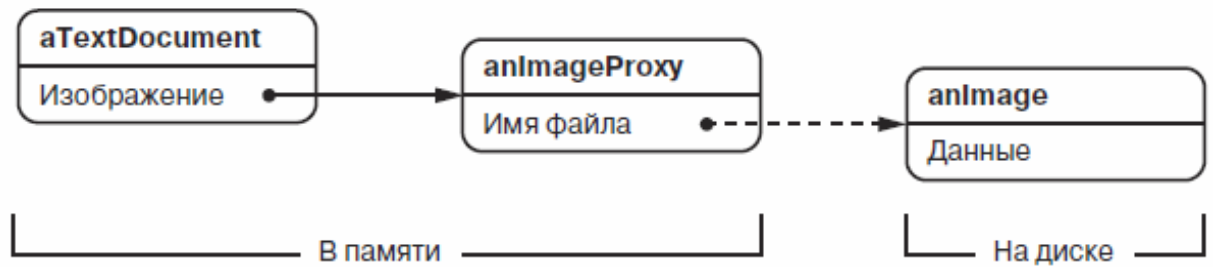
\includegraphics[width=0.6\textwidth]{proxyExample.png}
        \end{center}
    \end{frame}

    \begin{frame}
        \frametitle{Отложенная загрузка изображения}
        \begin{center}
            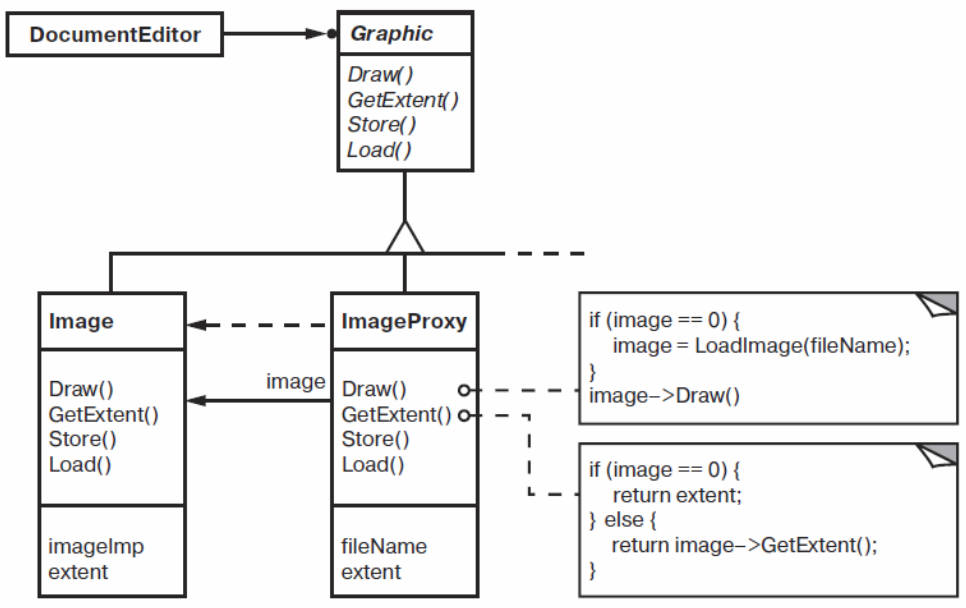
\includegraphics[width=0.7\textwidth]{proxyExampleClassDiagram.png}
        \end{center}
    \end{frame}

    \begin{frame}
        \frametitle{Паттерн <<Заместитель>>}
        \framesubtitle{Proxy}
        \begin{center}
            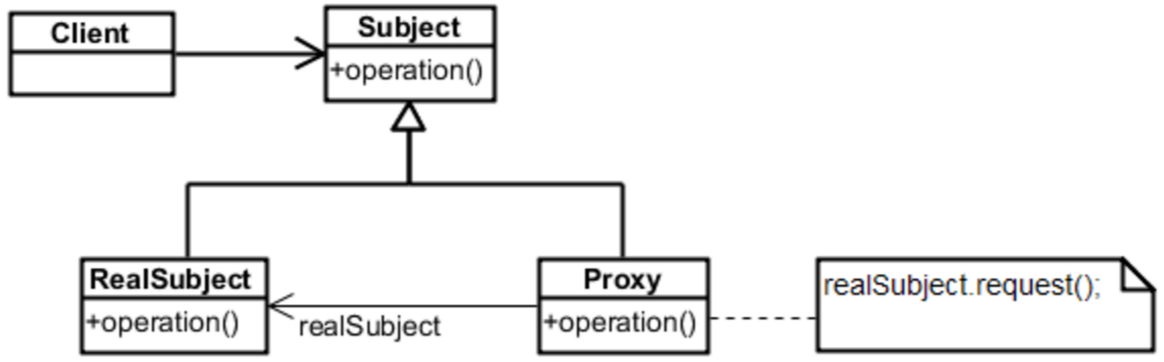
\includegraphics[width=0.6\textwidth]{proxy.png}
        \end{center}
        \begin{itemize}
            \item Замещение удалённых объектов
            \item Создание <<тяжёлых>> объектов по требованию
            \item Контроль доступа
            \item Умные указатели
            \begin{itemize}
                \item Подсчёт ссылок
                \item Ленивая загрузка/инициализация
                \item Работа с блокировками
                \item Копирование при записи
            \end{itemize}
        \end{itemize}
    \end{frame}

    \begin{frame}
        \frametitle{<<Заместитель>>, детали реализации}
        \begin{center}
            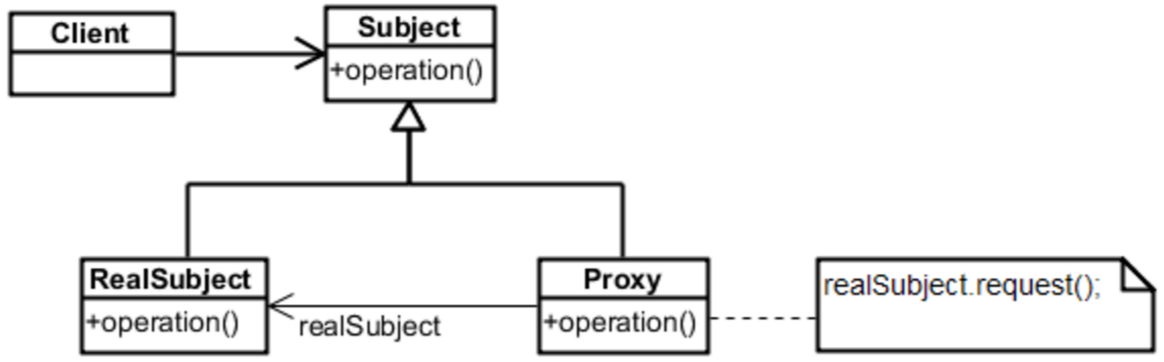
\includegraphics[width=0.6\textwidth]{proxy.png}
        \end{center}
        \begin{itemize}
            \item Перегрузка оператора доступа к членам класса (для C++)
            \begin{itemize}
                \item Умные указатели так устроены
                \item C++ вызывает операторы \mintinline{c++}|->| по цепочке
                \begin{itemize}
                    \item \mintinline{c++}|object->do()| может быть хоть \mintinline{c++}|((object.operator->()).operator->()).do()|
                \end{itemize}
                \item Не подходит, если надо различать операции
            \end{itemize}
        \end{itemize}
    \end{frame}

    \begin{frame}
        \frametitle{<<Заместитель>>, детали реализации (2)}
        \begin{itemize}
            \item Реализация <<вручную>> всех методов проксируемого объекта
            \begin{itemize}
                \item Сотня методов по одной строчке каждый
                \item C\#/F\#: \mintinline{csharp}|public void do() => realSubject.do();|
                \item Препроцессор/генерация
                \begin{itemize}
                    \item Технологии наподобие WCF
                \end{itemize}
            \end{itemize}
            \item Проксируемого объекта может не быть в памяти
        \end{itemize}
    \end{frame}

    \subsection{Паттерн <<Итератор>>}

    \begin{frame}
        \frametitle{<<Итератор>> (Iterator)}
        Инкапсулирует способ обхода коллекции.
        \begin{center}
            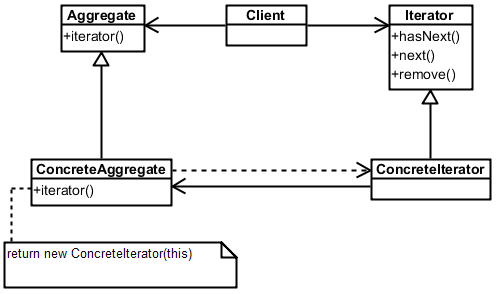
\includegraphics[width=0.6\textwidth]{iterator.png}
        \end{center}
        \begin{itemize}
            \item Разные итераторы для разных способов обхода
            \item Можно обходить не только коллекции
        \end{itemize}
    \end{frame}

    \begin{frame}[fragile]
        \frametitle{<<Итератор>>, примеры}
        \begin{itemize}
            \item Java-стиль:
            \begin{minted}{java}
public interface Iterator<E> {
    boolean hasNext();
    E next();
    void remove();
}
            \end{minted}
            \item .NET-стиль:
            \begin{minted}{csharp}
public interface IEnumerator<T>
{
    bool MoveNext();
    T Current { get; }
    void Reset();
}
            \end{minted}
        \end{itemize}
    \end{frame}

    \begin{frame}[fragile]
        \frametitle{<<Итератор>>, детали реализации (1)}
        \begin{itemize}
            \item Внешние итераторы
            \begin{minted}{csharp}
foreach (Thing t in collection)
{
    Console.WriteLine(t);
} 
            \end{minted}
            \item Внутренние итераторы
            \begin{minted}{csharp}
collection.ToList().ForEach(t => Console.WriteLine(t));
            \end{minted}
        \end{itemize}
    \end{frame}

    \begin{frame}
        \frametitle{<<Итератор>>, детали реализации (2)}
        \begin{itemize}
            \item Итераторы и курсоры
            \item Устойчивые и неустойчивые итераторы
            \begin{itemize}
                \item Паттерн <<Наблюдатель>>
                \item Даже обнаружение модификации коллекции может быть непросто
            \end{itemize}
            \item Дополнительные операции
        \end{itemize}
    \end{frame}

    \section{Архитектурные стили}

    \begin{frame}
        \frametitle{Архитектурные стили}
        \begin{itemize}
            \item Именованная коллекция архитектурных решений
            \item Менее узкоспециализированные, чем паттерны
            \item Определяют основные принципы построения системы в целом
        \end{itemize}
        \begin{center}
            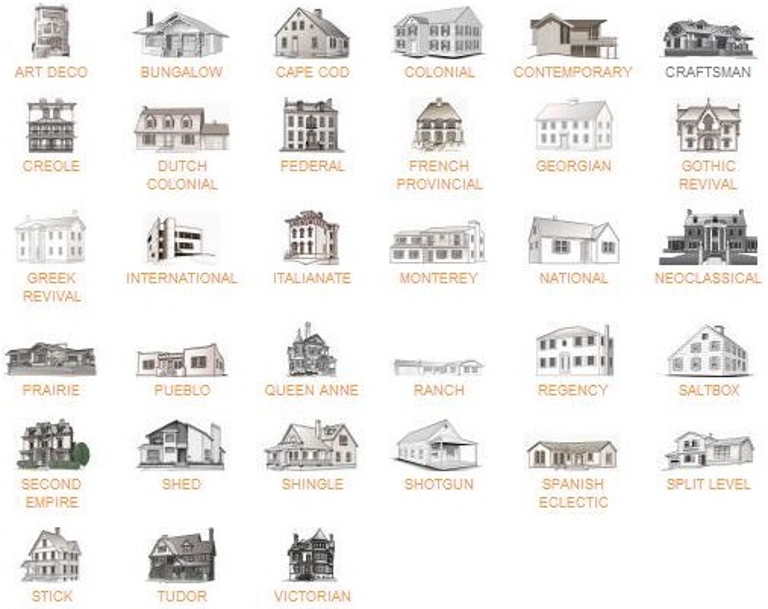
\includegraphics[width=0.5\textwidth]{buildingStyles.png}
            \attribution{N. Medvidovic}
        \end{center}
    \end{frame}

    \begin{frame}
        \frametitle{Архитектурные стили}
        \begin{columns}
            \begin{column}{0.5\textwidth}
                \begin{itemize}
                    \item Одна система может включать в себя несколько архитектурных стилей
                    \item Понятие стиля применимо и к подсистемам
                \end{itemize}
            \end{column}
            \begin{column}{0.5\textwidth}
                \begin{center}
                    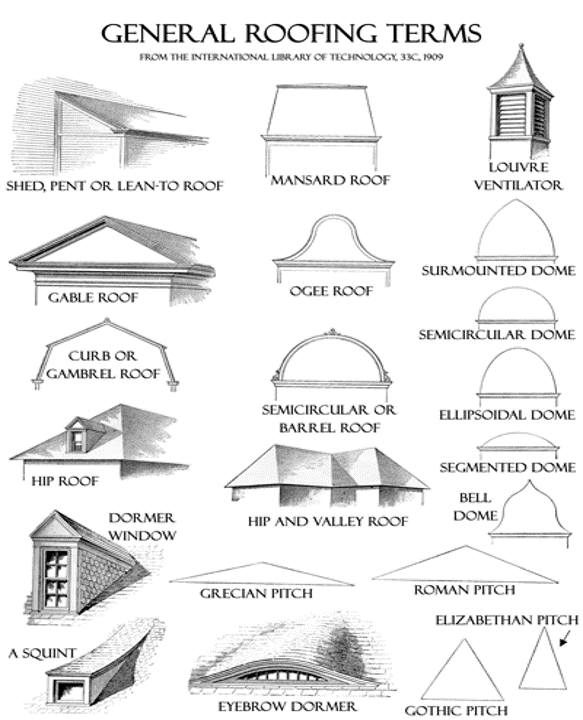
\includegraphics[width=0.7\textwidth]{roofStyles.png}
                    \attribution{N. Medvidovic}
                \end{center}
            \end{column}
        \end{columns}
    \end{frame}

    \subsection{Слоистый стиль}

    \begin{frame}
        \frametitle{Слоистый стиль}
        \framesubtitle{Layered style}
        \begin{itemize}
            \item Иерархическая организация системы
            \begin{itemize}
                \item Многоуровневый <<клиент-сервер>>
                \item Каждый слой предоставляет интерфейс для использования слоями выше
            \end{itemize}
            \item Каждый слой работает как:
            \begin{itemize}
                \item Сервер --- предоставляет функциональность слоям выше
                \item Клиент --- использует функциональность слоёв ниже
            \end{itemize}
            \item Пример --- операционные системы, сетевые стеки протоколов
        \end{itemize}
    \end{frame}

    \begin{frame}
        \frametitle{Слоистый стиль, подробности}
        \begin{columns}
            \begin{column}{0.5\textwidth}
                \begin{itemize}
                    \item Преимущества:
                    \begin{itemize}
                        \item Повышение уровня абстракции
                        \item Лёгкость в расширении
                        \item Изменения в каждом уровне затрагивают максимум два соседних
                        \item Возможны разные реализации уровня, если они удовлетворяют интерфейсу
                    \end{itemize}
                    \item Недостатки:
                    \begin{itemize}
                        \item Не всегда применим
                        \item Проблемы с производительностью
                    \end{itemize}
                \end{itemize}
            \end{column}
            \begin{column}{0.5\textwidth}
                \begin{center}
                    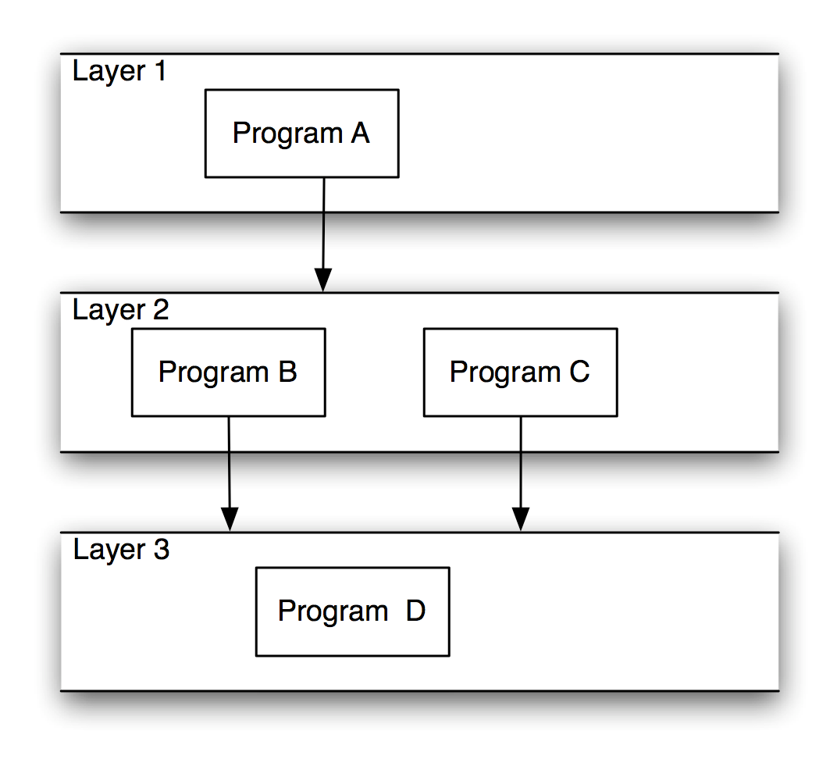
\includegraphics[width=0.8\textwidth]{layered.png}
                    \attribution{N. Medvidovic}
                \end{center}
            \end{column}
        \end{columns}
    \end{frame}

    \subsection{Каналы и фильтры}

    \begin{frame}
        \frametitle{Каналы и фильтры}
        \framesubtitle{Pipes and filters}
        \begin{itemize}
            \item Компоненты --- это фильтры, преобразующие данные из входных каналов в данные в выходных каналах
            \item Инварианты:
            \begin{itemize}
                \item Фильтры независимы (не имеют разделяемого состояния)
                \item Фильтры не знают о фильтрах до или после них
            \end{itemize}
            \item Вариации:
            \begin{itemize}
                \item Конвейеры --- линейные последовательности фильтров
                \item Ограниченные каналы --- где канал это очередь с ограниченным количеством элементов
                \item Типизированные каналы --- где каналы отличаются по типу передаваемых данных
            \end{itemize}
        \end{itemize}
    \end{frame}

    \begin{frame}
        \frametitle{Каналы и фильтры, подробности}
        \begin{itemize}
            \item Преимущества:
            \begin{itemize}
                \item Поведение системы --- это просто последовательное применение поведений компонентов
                \item Легко добавлять, заменять и переиспользовать фильтры
                \begin{itemize}
                    \item Любые два фильтра можно использовать вместе
                \end{itemize}
                \item Широкие возможности для анализа
                \begin{itemize}
                    \item Пропускная способность, задержки, deadlock-и
                \end{itemize}
                \item Широкие возможности для параллелизма
            \end{itemize}
            \item Недостатки:
            \begin{itemize}
                \item Последовательное исполнение
                \item Проблемы с интерактивными приложениями
                \item Пропускная способность определяется самым <<узким>> элементом
            \end{itemize}
        \end{itemize}
    \end{frame}

    \subsection{Стили с неявным вызовом}

    \begin{frame}
        \frametitle{Стили с неявным вызовом}
        \begin{itemize}
            \item Оповещение о событии вместо явного вызова метода
            \begin{itemize}
                \item Слушатели могут подписаться на событие
                \item Система при наступлении события сама вызывает все зарегистрированные методы слушателей
            \end{itemize}
            \item Компоненты имеют два вида интерфейсов --- методы и события
            \item Два типа соединителей:
            \begin{itemize}
                \item Явный вызов метода
                \item Неявный вызов по наступлению события
            \end{itemize}
            \item Инварианты:
            \begin{itemize}
                \item Те, кто производит события, не знают, кто и как на них отреагирует
                \item Не делается никаких предположений о том, как событие будет обработано и будет ли вообще
            \end{itemize}
        \end{itemize}
    \end{frame}

    \begin{frame}
        \frametitle{Стили с неявным вызовом, преимущества и недостатки}
        \begin{itemize}
            \item Преимущества:
            \begin{itemize}
                \item Переиспользование компонентов
                \begin{itemize}
                    \item Очень низкая связность между компонентами
                \end{itemize}
                \item Лёгкость в конфигурировании системы
                \begin{itemize}
                    \item Как во время компиляции, так и во время выполнения
                \end{itemize}
            \end{itemize}
            \item Недостатки:
            \begin{itemize}
                \item Зачастую неинтуитивная структура системы
                \item Компоненты не управляют последовательностью вычислений
                \item Непонятно, кто отреагирует на запрос и в каком порядке придут ответы
                \item Тяжело отлаживаться
                \item Гонки даже в однопоточном приложении
            \end{itemize}
        \end{itemize}
    \end{frame}

    \subsection{Peer-to-peer}

    \begin{frame}
        \frametitle{Peer-to-peer}
        \begin{itemize}
            \item Состояние и поведение распределены между компонентами, которые могут выступать как клиенты и как серверы
            \item Компоненты: имеют своё состояние и свой поток управления
            \item Соединители: как правило, сетевые протоколы
            \item Элементы данных: сетевые сообщения
            \item Топология: сеть (возможно, с избыточными связями между компонентами), может динамически меняться
            \item Преимущества:
            \begin{itemize}
                \item Хорош для распределённых вычислений
                \item Устойчив к отказам
                \item Если протокол взаимодействия позволяет, легко масштабируется
            \end{itemize}
        \end{itemize}
    \end{frame}

\end{document}
